% SOURCE: edit-harness/results/quant_survival/aggregate/gate_readout.json
% SOURCE FIELDS F10-A: thresholds.rank_survival_4bit; cells.{Llama-3.2-1B_rome_L12,Llama-3.2-3B_rome_L24}.arms.nf4dq_full_model.rho_damage_fp32_vs_arm_rank_survival_mean; gates.K1_geometry_ranking_survival.*.
% SOURCE FIELDS F10-B: thresholds.esr_survival_4bit; gates.K2_esr_survival_4bit.*; cells.{Llama-3.2-1B_rome_L12,Qwen2.5-1.5B_rome_L21}.arms.{nf4dq_edited_layer,nf4dq_full_model}.esr_survival_given_fp32_worked_mean.
% SOURCE FIELDS F10-C: cells.{Llama-3.2-1B_rome_L12,Llama-3.2-3B_rome_L24}.c3.nf4dq.F_above_mean; gates.K3_M_concentration.legacy_sensitivity_observations.
% SOURCE F10-D: docs/plans/PREREG-PAPERB-QUANTSURVIVAL-DRAFT-2026-07-16.md sections C1--C3 and K1--K3; disclosure wording matches manuscript limitations but main.tex is not an input.
% !TEX encoding = UTF-8 Unicode
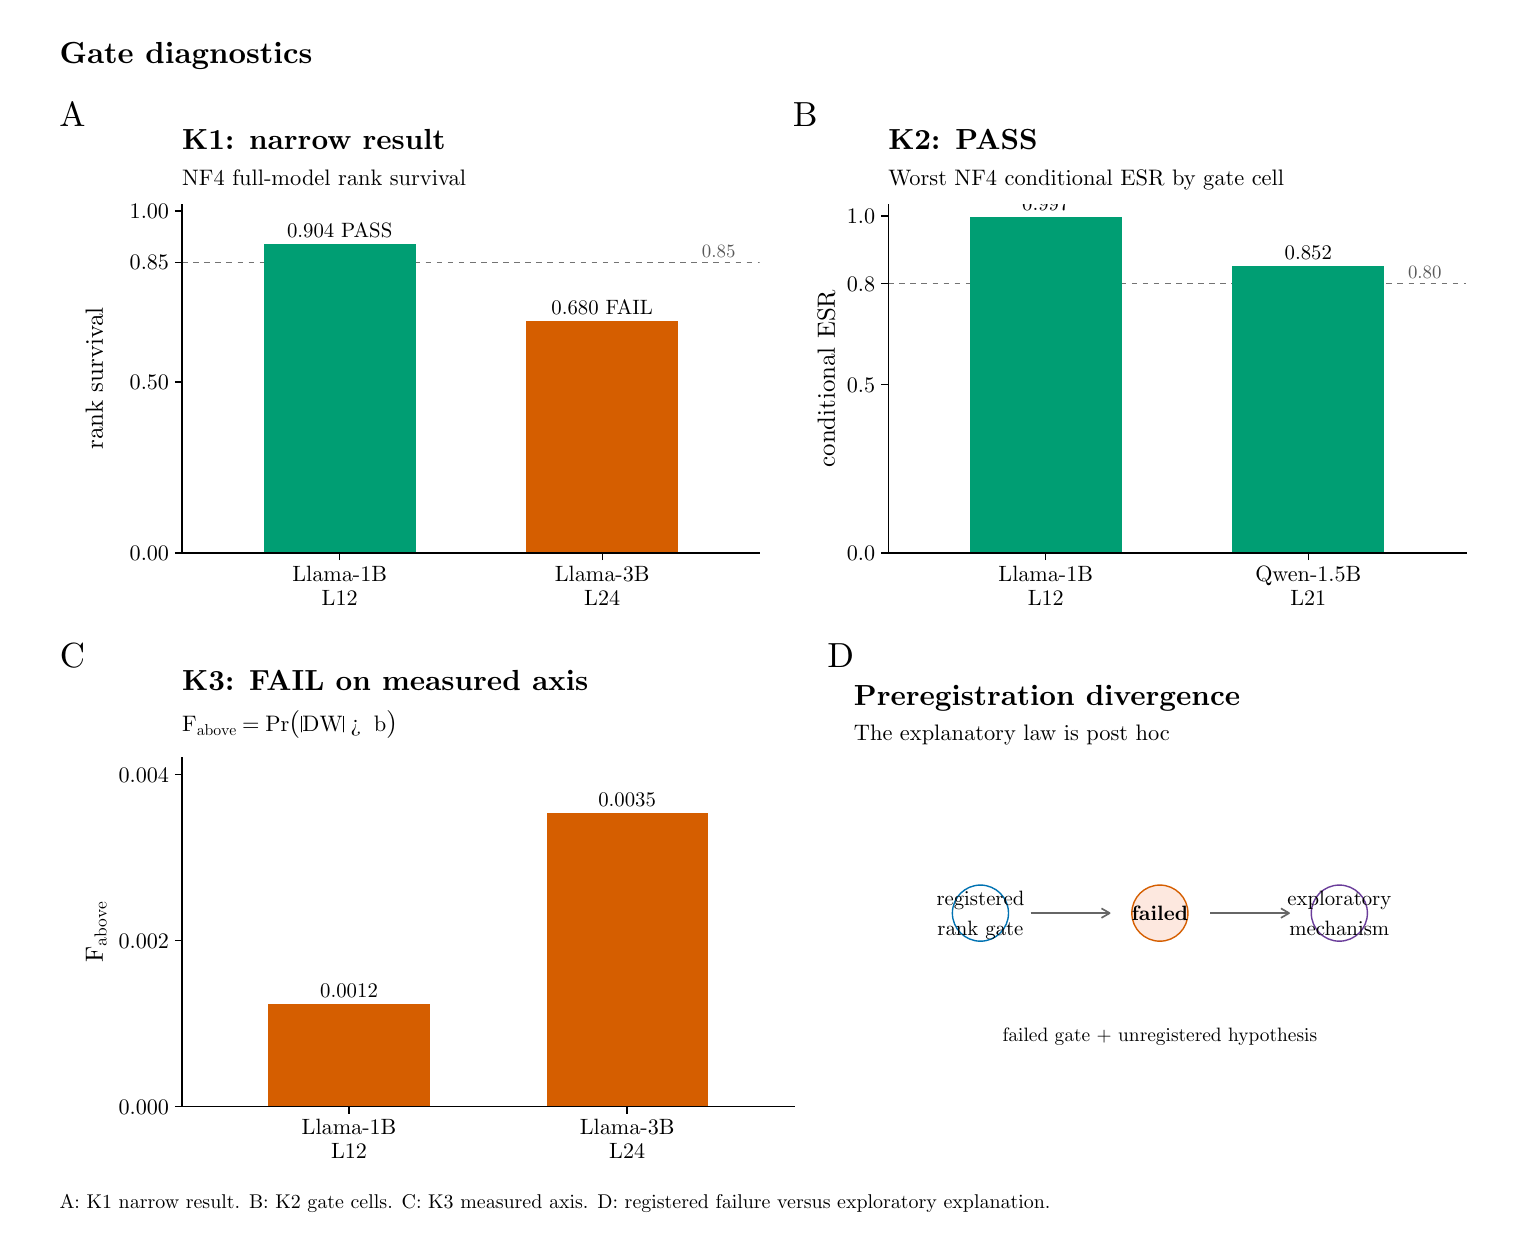
\begin{tikzpicture}[x=1pt,y=1pt]
\definecolor{fillColor}{RGB}{255,255,255}
\path[use as bounding box,fill=fillColor,fill opacity=0.00] (0,0) rectangle (531.18,433.62);
\begin{scope}
\path[clip] (  0.00,  0.00) rectangle (531.18,433.62);
\definecolor{drawColor}{RGB}{255,255,255}
\definecolor{fillColor}{RGB}{255,255,255}

\path[draw=drawColor,line width= 0.6pt,line join=round,line cap=round,fill=fillColor] (  0.00,  0.00) rectangle (531.18,433.62);
\end{scope}
\begin{scope}
\path[clip] (  5.50,217.39) rectangle (270.53,412.89);
\definecolor{drawColor}{RGB}{255,255,255}
\definecolor{fillColor}{RGB}{255,255,255}

\path[draw=drawColor,line width= 0.5pt,line join=round,line cap=round,fill=fillColor] (  5.50,217.39) rectangle (270.53,412.89);
\end{scope}
\begin{scope}
\path[clip] (270.53,217.39) rectangle (525.68,412.89);
\definecolor{drawColor}{RGB}{255,255,255}
\definecolor{fillColor}{RGB}{255,255,255}

\path[draw=drawColor,line width= 0.5pt,line join=round,line cap=round,fill=fillColor] (270.53,217.39) rectangle (525.68,412.89);
\end{scope}
\begin{scope}
\path[clip] ( 55.82,243.82) rectangle (264.53,369.82);
\definecolor{fillColor}{RGB}{255,255,255}

\path[fill=fillColor] ( 55.82,243.82) rectangle (264.53,369.82);
\definecolor{drawColor}{gray}{0.45}

\path[draw=drawColor,line width= 0.5pt,dash pattern=on 2pt off 2pt ,line join=round] ( 55.82,348.82) -- (264.53,348.82);
\definecolor{fillColor}{RGB}{0,158,115}

\path[fill=fillColor] ( 85.23,243.82) rectangle (140.25,355.47);
\definecolor{fillColor}{RGB}{213,94,0}

\path[fill=fillColor] (180.10,243.82) rectangle (235.12,327.79);
\definecolor{drawColor}{RGB}{0,0,0}

\node[text=drawColor,anchor=base,inner sep=0pt, outer sep=0pt, scale=  0.75] at (112.74,357.81) {0.904 PASS};

\node[text=drawColor,anchor=base,inner sep=0pt, outer sep=0pt, scale=  0.75] at (207.61,330.13) {0.680 FAIL};
\definecolor{drawColor}{gray}{0.35}

\node[text=drawColor,anchor=base west,inner sep=0pt, outer sep=0pt, scale=  0.68] at (243.66,350.47) {0.85};
\end{scope}
\begin{scope}
\path[clip] (  0.00,  0.00) rectangle (531.18,433.62);
\definecolor{drawColor}{RGB}{0,0,0}

\path[draw=drawColor,line width= 0.5pt,line join=round,line cap=rect] ( 55.82,243.82) --
	( 55.82,369.82);
\end{scope}
\begin{scope}
\path[clip] (  0.00,  0.00) rectangle (531.18,433.62);
\definecolor{drawColor}{RGB}{0,0,0}

\node[text=drawColor,anchor=base east,inner sep=0pt, outer sep=0pt, scale=  0.80] at ( 51.09,241.07) {0.00};

\node[text=drawColor,anchor=base east,inner sep=0pt, outer sep=0pt, scale=  0.80] at ( 51.09,302.83) {0.50};

\node[text=drawColor,anchor=base east,inner sep=0pt, outer sep=0pt, scale=  0.80] at ( 51.09,346.07) {0.85};

\node[text=drawColor,anchor=base east,inner sep=0pt, outer sep=0pt, scale=  0.80] at ( 51.09,364.60) {1.00};
\end{scope}
\begin{scope}
\path[clip] (  0.00,  0.00) rectangle (531.18,433.62);
\definecolor{drawColor}{RGB}{0,0,0}

\path[draw=drawColor,line width= 0.5pt,line join=round] ( 53.19,243.82) --
	( 55.82,243.82);

\path[draw=drawColor,line width= 0.5pt,line join=round] ( 53.19,305.59) --
	( 55.82,305.59);

\path[draw=drawColor,line width= 0.5pt,line join=round] ( 53.19,348.82) --
	( 55.82,348.82);

\path[draw=drawColor,line width= 0.5pt,line join=round] ( 53.19,367.35) --
	( 55.82,367.35);
\end{scope}
\begin{scope}
\path[clip] (  0.00,  0.00) rectangle (531.18,433.62);
\definecolor{drawColor}{RGB}{0,0,0}

\path[draw=drawColor,line width= 0.5pt,line join=round,line cap=rect] ( 55.82,243.82) --
	(264.53,243.82);
\end{scope}
\begin{scope}
\path[clip] (  0.00,  0.00) rectangle (531.18,433.62);
\definecolor{drawColor}{RGB}{0,0,0}

\path[draw=drawColor,line width= 0.5pt,line join=round] (112.74,241.20) --
	(112.74,243.82);

\path[draw=drawColor,line width= 0.5pt,line join=round] (207.61,241.20) --
	(207.61,243.82);
\end{scope}
\begin{scope}
\path[clip] (  0.00,  0.00) rectangle (531.18,433.62);
\definecolor{drawColor}{RGB}{0,0,0}

\node[text=drawColor,anchor=base,inner sep=0pt, outer sep=0pt, scale=  0.80] at (112.74,233.59) {Llama-1B};

\node[text=drawColor,anchor=base,inner sep=0pt, outer sep=0pt, scale=  0.80] at (112.74,224.95) {L12};

\node[text=drawColor,anchor=base,inner sep=0pt, outer sep=0pt, scale=  0.80] at (207.61,233.59) {Llama-3B};

\node[text=drawColor,anchor=base,inner sep=0pt, outer sep=0pt, scale=  0.80] at (207.61,224.95) {L24};
\end{scope}
\begin{scope}
\path[clip] (  0.00,  0.00) rectangle (531.18,433.62);
\definecolor{drawColor}{RGB}{0,0,0}

\node[text=drawColor,rotate= 90.00,anchor=base,inner sep=0pt, outer sep=0pt, scale=  0.90] at ( 27.15,306.82) {rank survival};
\end{scope}
\begin{scope}
\path[clip] (  0.00,  0.00) rectangle (531.18,433.62);
\definecolor{drawColor}{RGB}{0,0,0}

\node[text=drawColor,anchor=base west,inner sep=0pt, outer sep=0pt, scale=  0.81] at ( 55.82,376.65) {NF4 full-model rank survival};
\end{scope}
\begin{scope}
\path[clip] (  0.00,  0.00) rectangle (531.18,433.62);
\definecolor{drawColor}{RGB}{0,0,0}

\node[text=drawColor,anchor=base west,inner sep=0pt, outer sep=0pt, scale=  1.05] at ( 55.82,389.52) {\bfseries K1: narrow result};
\end{scope}
\begin{scope}
\path[clip] (  0.00,  0.00) rectangle (531.18,433.62);
\definecolor{drawColor}{RGB}{0,0,0}

\node[text=drawColor,anchor=base,inner sep=0pt, outer sep=0pt, scale=  1.26] at ( 16.22,397.99) {A};
\end{scope}
\begin{scope}
\path[clip] (310.97,243.82) rectangle (519.68,369.82);
\definecolor{fillColor}{RGB}{255,255,255}

\path[fill=fillColor] (310.97,243.82) rectangle (519.68,369.82);
\definecolor{drawColor}{gray}{0.45}

\path[draw=drawColor,line width= 0.5pt,dash pattern=on 2pt off 2pt ,line join=round] (310.97,341.21) -- (519.68,341.21);
\definecolor{fillColor}{RGB}{0,158,115}

\path[fill=fillColor] (340.38,243.82) rectangle (395.41,365.15);

\path[fill=fillColor] (435.25,243.82) rectangle (490.28,347.58);
\definecolor{drawColor}{RGB}{0,0,0}

\node[text=drawColor,anchor=base,inner sep=0pt, outer sep=0pt, scale=  0.75] at (367.89,367.49) {0.997};

\node[text=drawColor,anchor=base,inner sep=0pt, outer sep=0pt, scale=  0.75] at (462.76,349.92) {0.852};
\definecolor{drawColor}{gray}{0.35}

\node[text=drawColor,anchor=base west,inner sep=0pt, outer sep=0pt, scale=  0.68] at (498.81,342.86) {0.80};
\end{scope}
\begin{scope}
\path[clip] (  0.00,  0.00) rectangle (531.18,433.62);
\definecolor{drawColor}{RGB}{0,0,0}

\path[draw=drawColor,line width= 0.5pt,line join=round,line cap=rect] (310.97,243.82) --
	(310.97,369.82);
\end{scope}
\begin{scope}
\path[clip] (  0.00,  0.00) rectangle (531.18,433.62);
\definecolor{drawColor}{RGB}{0,0,0}

\node[text=drawColor,anchor=base east,inner sep=0pt, outer sep=0pt, scale=  0.80] at (306.25,241.07) {0.0};

\node[text=drawColor,anchor=base east,inner sep=0pt, outer sep=0pt, scale=  0.80] at (306.25,301.94) {0.5};

\node[text=drawColor,anchor=base east,inner sep=0pt, outer sep=0pt, scale=  0.80] at (306.25,338.46) {0.8};

\node[text=drawColor,anchor=base east,inner sep=0pt, outer sep=0pt, scale=  0.80] at (306.25,362.81) {1.0};
\end{scope}
\begin{scope}
\path[clip] (  0.00,  0.00) rectangle (531.18,433.62);
\definecolor{drawColor}{RGB}{0,0,0}

\path[draw=drawColor,line width= 0.5pt,line join=round] (308.35,243.82) --
	(310.97,243.82);

\path[draw=drawColor,line width= 0.5pt,line join=round] (308.35,304.69) --
	(310.97,304.69);

\path[draw=drawColor,line width= 0.5pt,line join=round] (308.35,341.21) --
	(310.97,341.21);

\path[draw=drawColor,line width= 0.5pt,line join=round] (308.35,365.56) --
	(310.97,365.56);
\end{scope}
\begin{scope}
\path[clip] (  0.00,  0.00) rectangle (531.18,433.62);
\definecolor{drawColor}{RGB}{0,0,0}

\path[draw=drawColor,line width= 0.5pt,line join=round,line cap=rect] (310.97,243.82) --
	(519.68,243.82);
\end{scope}
\begin{scope}
\path[clip] (  0.00,  0.00) rectangle (531.18,433.62);
\definecolor{drawColor}{RGB}{0,0,0}

\path[draw=drawColor,line width= 0.5pt,line join=round] (367.89,241.20) --
	(367.89,243.82);

\path[draw=drawColor,line width= 0.5pt,line join=round] (462.76,241.20) --
	(462.76,243.82);
\end{scope}
\begin{scope}
\path[clip] (  0.00,  0.00) rectangle (531.18,433.62);
\definecolor{drawColor}{RGB}{0,0,0}

\node[text=drawColor,anchor=base,inner sep=0pt, outer sep=0pt, scale=  0.80] at (367.89,233.59) {Llama-1B};

\node[text=drawColor,anchor=base,inner sep=0pt, outer sep=0pt, scale=  0.80] at (367.89,224.95) {L12};

\node[text=drawColor,anchor=base,inner sep=0pt, outer sep=0pt, scale=  0.80] at (462.76,233.59) {Qwen-1.5B};

\node[text=drawColor,anchor=base,inner sep=0pt, outer sep=0pt, scale=  0.80] at (462.76,224.95) {L21};
\end{scope}
\begin{scope}
\path[clip] (  0.00,  0.00) rectangle (531.18,433.62);
\definecolor{drawColor}{RGB}{0,0,0}

\node[text=drawColor,rotate= 90.00,anchor=base,inner sep=0pt, outer sep=0pt, scale=  0.90] at (291.65,306.82) {conditional ESR};
\end{scope}
\begin{scope}
\path[clip] (  0.00,  0.00) rectangle (531.18,433.62);
\definecolor{drawColor}{RGB}{0,0,0}

\node[text=drawColor,anchor=base west,inner sep=0pt, outer sep=0pt, scale=  0.81] at (310.97,376.65) {Worst NF4 conditional ESR by gate cell};
\end{scope}
\begin{scope}
\path[clip] (  0.00,  0.00) rectangle (531.18,433.62);
\definecolor{drawColor}{RGB}{0,0,0}

\node[text=drawColor,anchor=base west,inner sep=0pt, outer sep=0pt, scale=  1.05] at (310.97,389.52) {\bfseries K2: PASS};
\end{scope}
\begin{scope}
\path[clip] (  0.00,  0.00) rectangle (531.18,433.62);
\definecolor{drawColor}{RGB}{0,0,0}

\node[text=drawColor,anchor=base,inner sep=0pt, outer sep=0pt, scale=  1.26] at (280.99,397.99) {B};
\end{scope}
\begin{scope}
\path[clip] (  5.50, 17.36) rectangle (282.94,217.39);
\definecolor{drawColor}{RGB}{255,255,255}
\definecolor{fillColor}{RGB}{255,255,255}

\path[draw=drawColor,line width= 0.5pt,line join=round,line cap=round,fill=fillColor] (  5.50, 17.36) rectangle (282.94,217.39);
\end{scope}
\begin{scope}
\path[clip] (282.94, 17.36) rectangle (525.68,217.39);

\path[] (282.94, 17.36) rectangle (525.68,217.39);
\end{scope}
\begin{scope}
\path[clip] ( 55.82, 43.79) rectangle (276.94,169.79);
\definecolor{fillColor}{RGB}{255,255,255}

\path[fill=fillColor] ( 55.82, 43.79) rectangle (276.94,169.79);
\definecolor{fillColor}{RGB}{213,94,0}

\path[fill=fillColor] ( 86.98, 43.79) rectangle (145.27, 80.79);

\path[fill=fillColor] (187.49, 43.79) rectangle (245.78,149.79);
\definecolor{drawColor}{RGB}{0,0,0}

\node[text=drawColor,anchor=base,inner sep=0pt, outer sep=0pt, scale=  0.75] at (116.13, 83.12) {0.0012};

\node[text=drawColor,anchor=base,inner sep=0pt, outer sep=0pt, scale=  0.75] at (216.63,152.12) {0.0035};
\end{scope}
\begin{scope}
\path[clip] (  0.00,  0.00) rectangle (531.18,433.62);
\definecolor{drawColor}{RGB}{0,0,0}

\path[draw=drawColor,line width= 0.5pt,line join=round,line cap=rect] ( 55.82, 43.79) --
	( 55.82,169.79);
\end{scope}
\begin{scope}
\path[clip] (  0.00,  0.00) rectangle (531.18,433.62);
\definecolor{drawColor}{RGB}{0,0,0}

\node[text=drawColor,anchor=base east,inner sep=0pt, outer sep=0pt, scale=  0.80] at ( 51.09, 41.03) {0.000};

\node[text=drawColor,anchor=base east,inner sep=0pt, outer sep=0pt, scale=  0.80] at ( 51.09,101.03) {0.002};

\node[text=drawColor,anchor=base east,inner sep=0pt, outer sep=0pt, scale=  0.80] at ( 51.09,161.03) {0.004};
\end{scope}
\begin{scope}
\path[clip] (  0.00,  0.00) rectangle (531.18,433.62);
\definecolor{drawColor}{RGB}{0,0,0}

\path[draw=drawColor,line width= 0.5pt,line join=round] ( 53.19, 43.79) --
	( 55.82, 43.79);

\path[draw=drawColor,line width= 0.5pt,line join=round] ( 53.19,103.79) --
	( 55.82,103.79);

\path[draw=drawColor,line width= 0.5pt,line join=round] ( 53.19,163.79) --
	( 55.82,163.79);
\end{scope}
\begin{scope}
\path[clip] (  0.00,  0.00) rectangle (531.18,433.62);
\definecolor{drawColor}{RGB}{0,0,0}

\path[draw=drawColor,line width= 0.5pt,line join=round,line cap=rect] ( 55.82, 43.79) --
	(276.94, 43.79);
\end{scope}
\begin{scope}
\path[clip] (  0.00,  0.00) rectangle (531.18,433.62);
\definecolor{drawColor}{RGB}{0,0,0}

\path[draw=drawColor,line width= 0.5pt,line join=round] (116.13, 41.16) --
	(116.13, 43.79);

\path[draw=drawColor,line width= 0.5pt,line join=round] (216.63, 41.16) --
	(216.63, 43.79);
\end{scope}
\begin{scope}
\path[clip] (  0.00,  0.00) rectangle (531.18,433.62);
\definecolor{drawColor}{RGB}{0,0,0}

\node[text=drawColor,anchor=base,inner sep=0pt, outer sep=0pt, scale=  0.80] at (116.13, 33.55) {Llama-1B};

\node[text=drawColor,anchor=base,inner sep=0pt, outer sep=0pt, scale=  0.80] at (116.13, 24.91) {L12};

\node[text=drawColor,anchor=base,inner sep=0pt, outer sep=0pt, scale=  0.80] at (216.63, 33.55) {Llama-3B};

\node[text=drawColor,anchor=base,inner sep=0pt, outer sep=0pt, scale=  0.80] at (216.63, 24.91) {L24};
\end{scope}
\begin{scope}
\path[clip] (  0.00,  0.00) rectangle (531.18,433.62);
\definecolor{drawColor}{RGB}{0,0,0}

\node[text=drawColor,rotate= 90.00,anchor=base west,inner sep=0pt, outer sep=0pt, scale=  0.90] at ( 27.15, 95.89) {F};

\node[text=drawColor,rotate= 90.00,anchor=base west,inner sep=0pt, outer sep=0pt, scale=  0.63] at ( 28.50,101.76) {a};

\node[text=drawColor,rotate= 90.00,anchor=base west,inner sep=0pt, outer sep=0pt, scale=  0.63] at ( 28.50,104.91) {b};

\node[text=drawColor,rotate= 90.00,anchor=base west,inner sep=0pt, outer sep=0pt, scale=  0.63] at ( 28.50,108.41) {o};

\node[text=drawColor,rotate= 90.00,anchor=base west,inner sep=0pt, outer sep=0pt, scale=  0.63] at ( 28.50,111.56) {v};

\node[text=drawColor,rotate= 90.00,anchor=base west,inner sep=0pt, outer sep=0pt, scale=  0.63] at ( 28.50,114.89) {e};
\end{scope}
\begin{scope}
\path[clip] (  0.00,  0.00) rectangle (531.18,433.62);
\definecolor{drawColor}{RGB}{0,0,0}

\node[text=drawColor,anchor=base west,inner sep=0pt, outer sep=0pt, scale=  0.81] at ( 55.82,179.14) {F};

\node[text=drawColor,anchor=base west,inner sep=0pt, outer sep=0pt, scale=  0.57] at ( 61.11,177.92) {a};

\node[text=drawColor,anchor=base west,inner sep=0pt, outer sep=0pt, scale=  0.57] at ( 63.94,177.92) {b};

\node[text=drawColor,anchor=base west,inner sep=0pt, outer sep=0pt, scale=  0.57] at ( 67.09,177.92) {o};

\node[text=drawColor,anchor=base west,inner sep=0pt, outer sep=0pt, scale=  0.57] at ( 69.92,177.92) {v};

\node[text=drawColor,anchor=base west,inner sep=0pt, outer sep=0pt, scale=  0.57] at ( 72.92,177.92) {e};

\node[text=drawColor,anchor=base west,inner sep=0pt, outer sep=0pt, scale=  0.81] at ( 77.50,179.14) {=};

\node[text=drawColor,anchor=base west,inner sep=0pt, outer sep=0pt, scale=  0.81] at ( 85.86,179.14) {Pr};

\node[text=drawColor,anchor=base west,inner sep=0pt, outer sep=0pt, scale=  1.01] at ( 94.54,179.14) {(};

\path[draw=drawColor,line width= 0.4pt,line join=round,line cap=round] ( 98.89,179.14) --
	( 98.89,184.72);

\node[text=drawColor,anchor=base west,inner sep=0pt, outer sep=0pt, scale=  0.81] at ( 99.30,179.14) {D};

\node[text=drawColor,anchor=base west,inner sep=0pt, outer sep=0pt, scale=  0.81] at (105.49,179.14) {W};

\path[draw=drawColor,line width= 0.4pt,line join=round,line cap=round] (114.22,179.14) --
	(114.22,184.72);

\node[text=drawColor,anchor=base west,inner sep=0pt, outer sep=0pt, scale=  0.81] at (116.69,179.14) {>};

\node[text=drawColor,anchor=base west,inner sep=0pt, outer sep=0pt, scale=  0.81] at (125.06,179.14) {b};

\node[text=drawColor,anchor=base west,inner sep=0pt, outer sep=0pt, scale=  1.01] at (129.55,179.14) {)};
\end{scope}
\begin{scope}
\path[clip] (  0.00,  0.00) rectangle (531.18,433.62);
\definecolor{drawColor}{RGB}{0,0,0}

\node[text=drawColor,anchor=base west,inner sep=0pt, outer sep=0pt, scale=  1.05] at ( 55.82,194.02) {\bfseries K3: FAIL on measured axis};
\end{scope}
\begin{scope}
\path[clip] (  0.00,  0.00) rectangle (531.18,433.62);
\definecolor{drawColor}{RGB}{0,0,0}

\node[text=drawColor,anchor=base,inner sep=0pt, outer sep=0pt, scale=  1.26] at ( 16.22,202.49) {C};
\end{scope}
\begin{scope}
\path[clip] (  0.00,  0.00) rectangle (531.18,433.62);
\definecolor{drawColor}{gray}{0.40}

\path[draw=drawColor,line width= 0.6pt,line join=round] (362.44,113.66) -- (390.97,113.66);

\path[draw=drawColor,line width= 0.6pt,line join=round] (388.01,111.95) --
	(390.97,113.66) --
	(388.01,115.37);

\path[draw=drawColor,line width= 0.6pt,line join=round] (427.28,113.66) -- (455.81,113.66);

\path[draw=drawColor,line width= 0.6pt,line join=round] (452.86,111.95) --
	(455.81,113.66) --
	(452.86,115.37);
\definecolor{drawColor}{RGB}{0,114,178}
\definecolor{fillColor}{RGB}{255,255,255}

\path[draw=drawColor,line width= 0.5pt,line join=round,line cap=round,fill=fillColor] (344.28,113.66) circle ( 10.14);
\definecolor{drawColor}{RGB}{213,94,0}
\definecolor{fillColor}{RGB}{253,232,223}

\path[draw=drawColor,line width= 0.5pt,line join=round,line cap=round,fill=fillColor] (409.12,113.66) circle ( 10.14);
\definecolor{drawColor}{RGB}{106,61,154}
\definecolor{fillColor}{RGB}{255,255,255}

\path[draw=drawColor,line width= 0.5pt,line join=round,line cap=round,fill=fillColor] (473.97,113.66) circle ( 10.14);
\definecolor{drawColor}{RGB}{0,0,0}

\node[text=drawColor,anchor=base,inner sep=0pt, outer sep=0pt, scale=  0.75] at (344.28,116.49) {registered};

\node[text=drawColor,anchor=base,inner sep=0pt, outer sep=0pt, scale=  0.75] at (344.28,105.64) {rank gate};

\node[text=drawColor,anchor=base,inner sep=0pt, outer sep=0pt, scale=  0.75] at (409.12,111.06) {\bfseries failed};

\node[text=drawColor,anchor=base,inner sep=0pt, outer sep=0pt, scale=  0.75] at (473.97,116.49) {exploratory};

\node[text=drawColor,anchor=base,inner sep=0pt, outer sep=0pt, scale=  0.75] at (473.97,105.64) {mechanism};

\node[text=drawColor,anchor=base,inner sep=0pt, outer sep=0pt, scale=  0.70] at (409.12, 67.27) {failed gate + unregistered hypothesis};
\end{scope}
\begin{scope}
\path[clip] (  0.00,  0.00) rectangle (531.18,433.62);
\definecolor{drawColor}{RGB}{0,0,0}

\node[text=drawColor,anchor=base west,inner sep=0pt, outer sep=0pt, scale=  0.81] at (298.56,175.90) {The explanatory law is post hoc};
\end{scope}
\begin{scope}
\path[clip] (  0.00,  0.00) rectangle (531.18,433.62);
\definecolor{drawColor}{RGB}{0,0,0}

\node[text=drawColor,anchor=base west,inner sep=0pt, outer sep=0pt, scale=  1.05] at (298.56,188.77) {\bfseries Preregistration divergence};
\end{scope}
\begin{scope}
\path[clip] (  0.00,  0.00) rectangle (531.18,433.62);
\definecolor{drawColor}{RGB}{0,0,0}

\node[text=drawColor,anchor=base,inner sep=0pt, outer sep=0pt, scale=  1.26] at (293.75,202.49) {D};
\end{scope}
\begin{scope}
\path[clip] (  0.00,  0.00) rectangle (531.18,433.62);
\definecolor{drawColor}{RGB}{0,0,0}

\node[text=drawColor,anchor=base west,inner sep=0pt, outer sep=0pt, scale=  0.72] at ( 11.50,  6.90) {A: K1 narrow result. B: K2 gate cells. C: K3 measured axis. D: registered failure versus exploratory explanation.};
\end{scope}
\begin{scope}
\path[clip] (  0.00,  0.00) rectangle (531.18,433.62);
\definecolor{drawColor}{RGB}{0,0,0}

\node[text=drawColor,anchor=base west,inner sep=0pt, outer sep=0pt, scale=  1.10] at ( 11.50,420.53) {\bfseries Gate diagnostics};
\end{scope}
\end{tikzpicture}
